\chapter{Experiments and Results}
    \label{chap:experiments}
    
    In this chapter, we introduce the experimental setup and explain the conducted experiments and the obtained results.
    
    \section{Experimental setup}
        For each experiment, the training set is divided into three partitions: $A$, $B$, and $C$, each one with a predetermined size. $A$ and $B$ partitions will be used as the initial labeled training set, while $C$ will be used as the large \emph{unlabeled} pool.
        
        
        In case the number of samples in the obtained training set is less than the size of the entire training set (i.e., $|A| + |B| + |C|$), \emph{resampling} is performed. This makes for a fair comparison between the different \acrshort{al} approaches.
        
        
        More in detail, experiments are conducted by training and testing 10 runs off an autoencoder the \acrshort{al} techniques explained in \autoref{sub:al}.
        %  \begin{itemize}
             \subsection*{AL1}
             This baseline model does not use any \acrshort{al} method. The model is trained only on the $A$ and $B$ partitions of the training set.
             
             \subsection*{AL2}
             This is our second baseline model, it randomly queries $n$ samples from partition $C$. The final model is trained on partitions $A$, $B$, and the newly sampled data.
             
             \subsection*{AL3.1}
             This approach trains an intermediate model ($AL1$) using only the $A$ and $B$ partitions. It then uses this model to query the most anomalous $n$ samples from $C$ to be included in the new training set for the model. The final model is trained on the new extended set.
             
             \subsection*{AL3.2}
             This approach works similarly to $AL3.1$, although it uses another intermediate model:
                \begin{enumerate}
                    \item the most anomalous $n/2$ samples (wrt AL1) from partition $C$ are queried;
                    \item an intermediate (AL-tmp) model is trained on this new expanded dataset;
                    \item the final dataset is obtained by the AL-tmp training set plus the $n/2$ most anomalous samples (wrt AL-tmp).
                \end{enumerate}
                
             \subsection*{AL4 to AL8}
             All these approaches use $AL1$ as intermediate model to query the $n$ most \emph{informative} samples from partition $C$ following the criteria shown in \autoref{sub:al}.
        %  \end{itemize}

    \section{Model exploration}

        Preliminary tests are conducted to check whether the models were learning correctly.
        
        
        These tests are conducted by both checking the AUC of the models in the test set and by visualizing the reconstructed images. Figures \ref{fig:pred-mnist}, \ref{fig:pred-rm} show model predictions for a \emph{normal} and an \emph{anomalous} sample. The model can reproduce any normal sample with little to no error. However, if the model receives an anomalous sample, it will not be capable of reconstructing it correctly. This results in the "brighter" anomaly map in both Figures.
        
        \begin{figure}[H]
                \centering
                \centerline{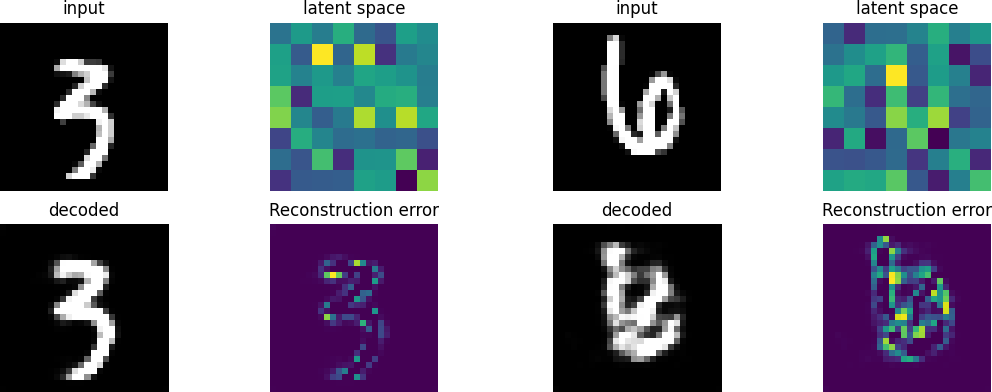
\includegraphics[width=\textwidth]{img/prediction_MNIST.png}}
                \caption{Example of predictions from a model trained on MNIST. The input image on the left is from the normal class, while the other on the right is anomalous}
                \label{fig:pred-mnist}
        \end{figure}
        
    % \subsection{Tests for models learning average}
    
        \subsection{Early phase}
        
            In an early phase, we studied models with extreme architectural characteristics such as an autoencoder with no bottleneck. This was done to study the bottleneck size hyperparameter for the MNIST dataset shown in \autoref{sub:bn}.
        
            % Models with a bottleneck size of 0 are used on MNIST to find out which bottleneck size is the best for the task. Models with a bottleneck size of 0 should learn an average representation of the training data. This is because the bottleneck layer is removed and the model is forced to learn the average representation of the training data.
    
            % Debug runs are necessary for these models because, for the first runs, they were not learning as expected. This is because in the first versions of the autoencoder when a bottleneck size of $0$ is used, the decoder receives a tensor filled with $0$ values. These values would nullify the weights of the decoder and the model would not learn anything, the only parameter it could learn is the bias. This problem is solved by feeding the decoder a tensor filled with $1$ values. This way the decoder would correctly learn the average representation of the training data.
        
        \subsection{Dummy models}
        
            We test some dummy models to check whether our model evaluation pipeline is working correctly. To test it we developed and deployed three dummy models:
            \begin{itemize}
                \item DummyFalse
                \item DummyTrue
                \item DummyRandom
            \end{itemize}
            
            The first model predicts any sample as \emph{normal}, and the second predicts everything as \emph{anomalous}. The third model randomly chooses between the two classes for any given input.
            
            As expected the AUC of DummyFalse and DummyTrue is 0.5. For DummyRandom the boxplot in \autoref{fig:pred-dummy} shows this model has an AUC score close to 0.5.
            
            \begin{figure}[H]
                \centering
                \centerline{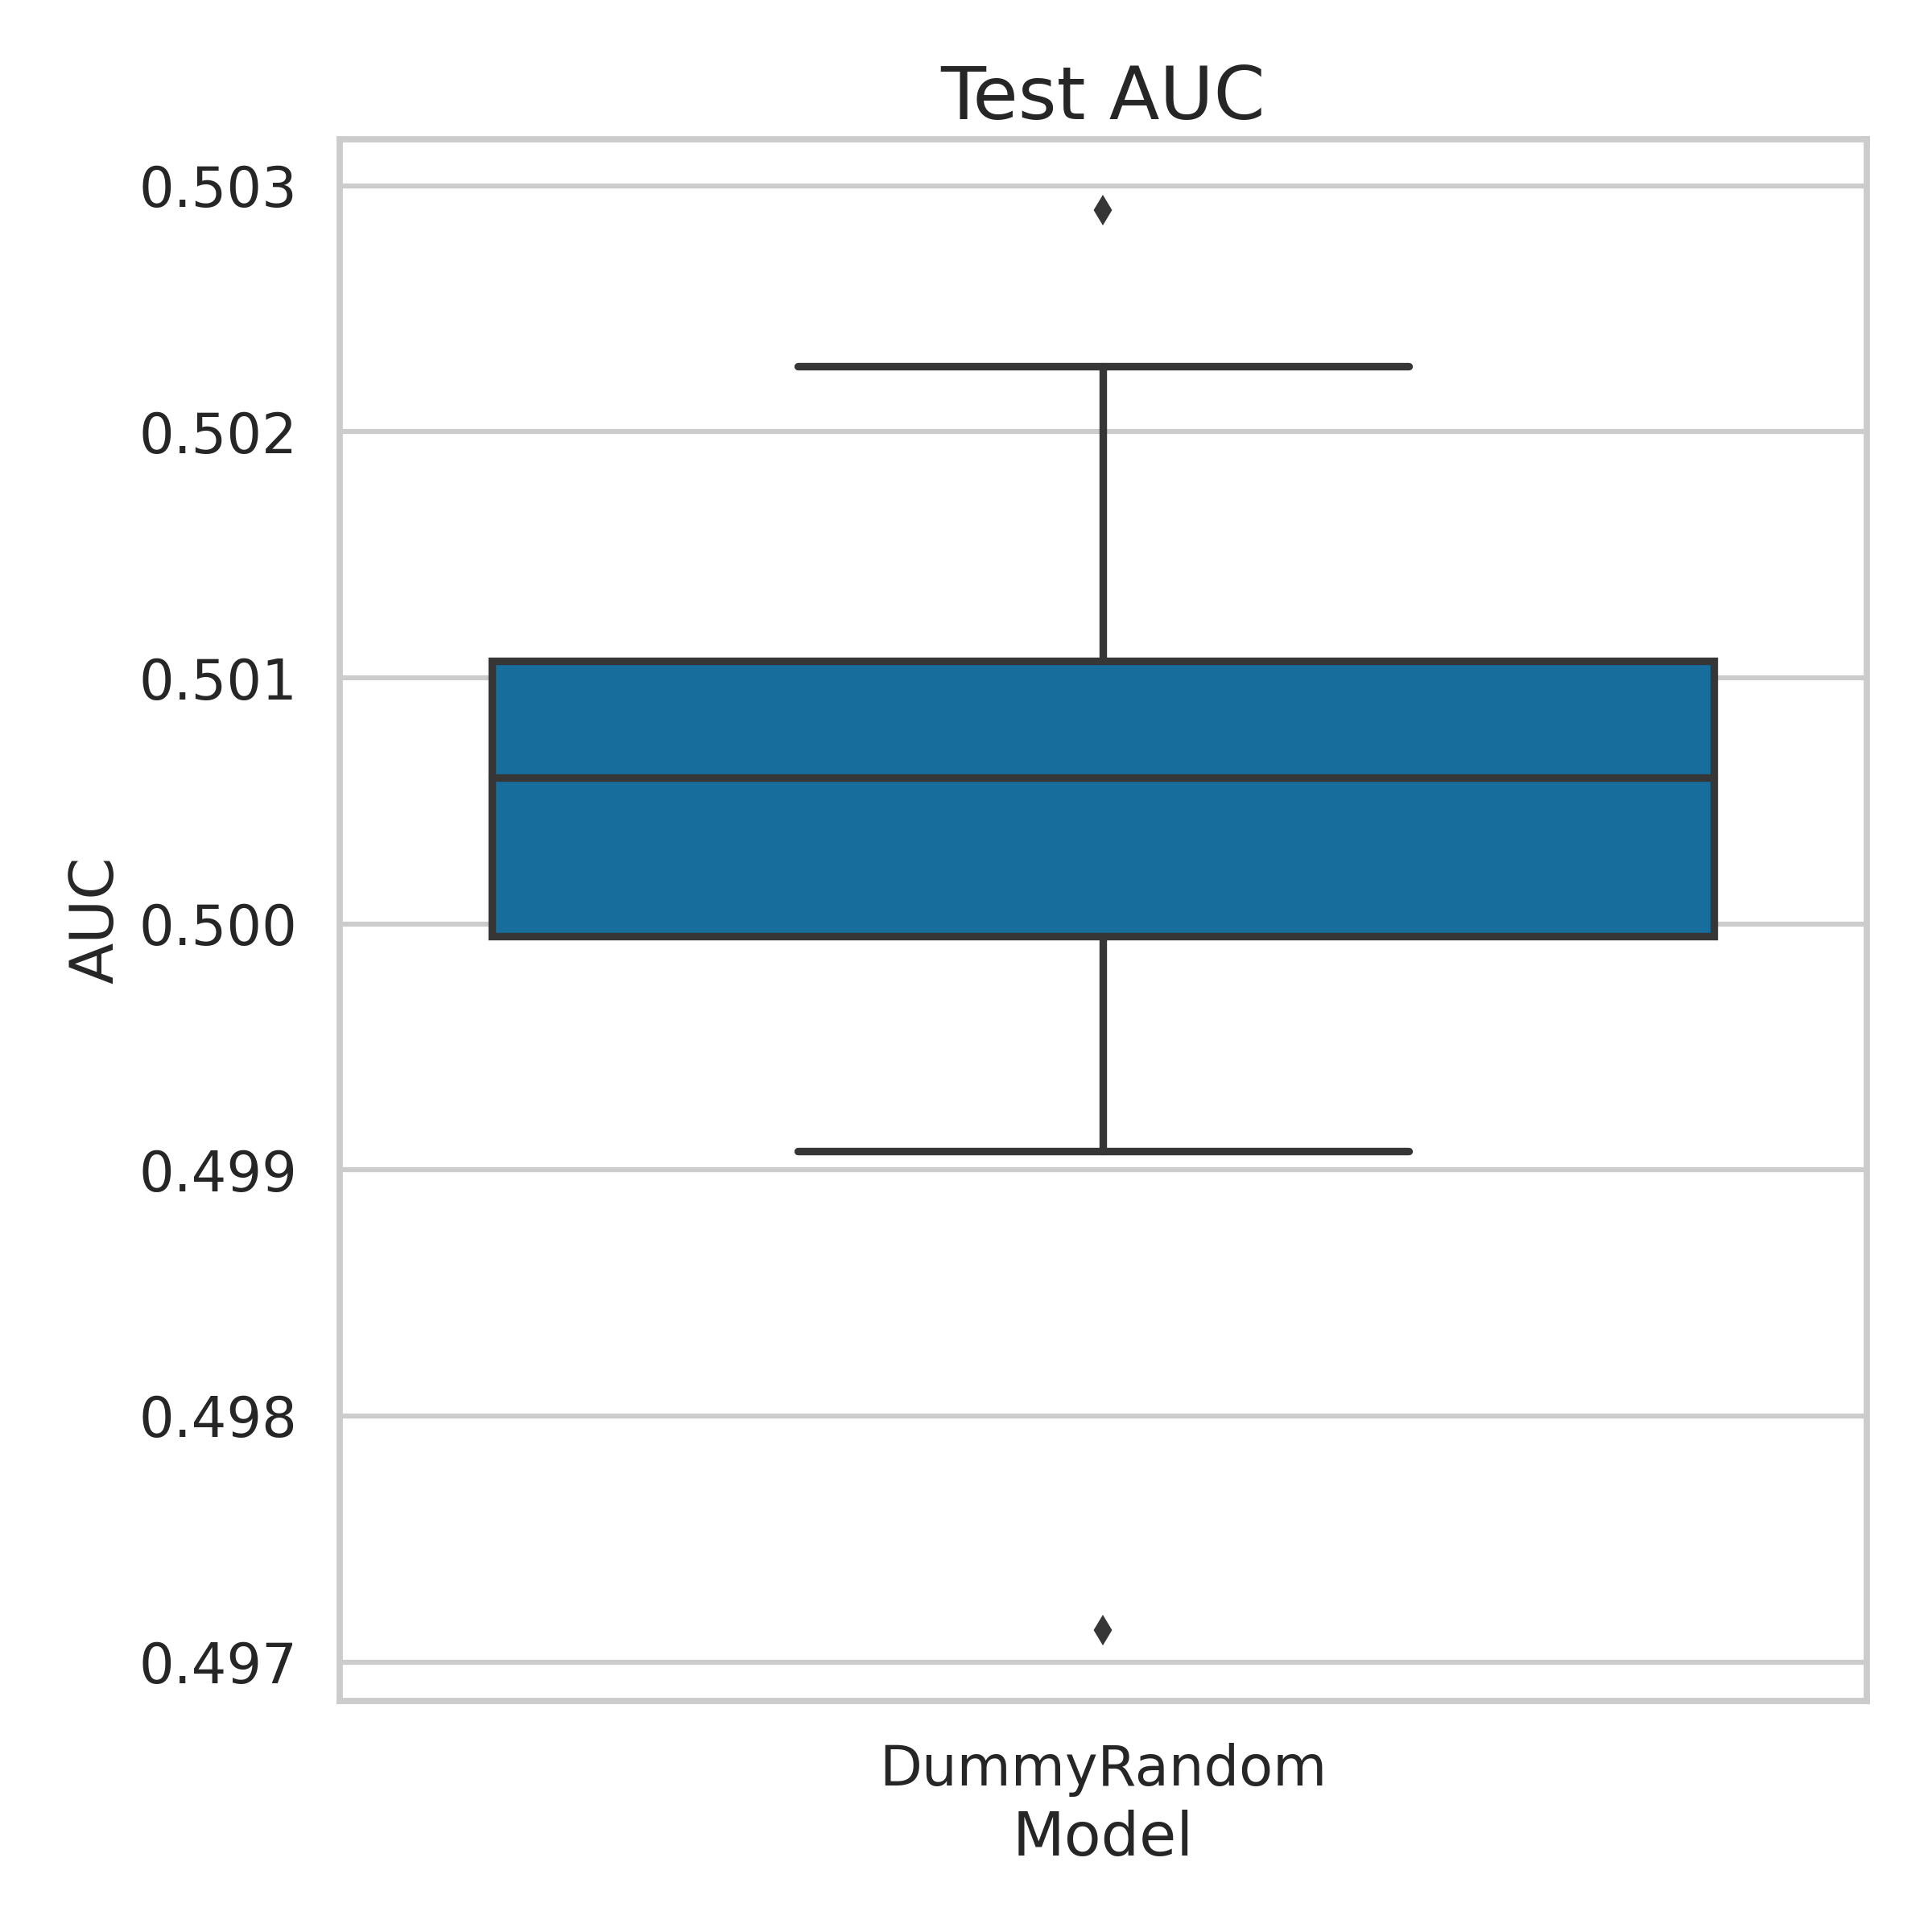
\includegraphics[width=0.5\textwidth]{img/results/dummy.png}}
                \caption{Test AUC for DummyRandom model, boxplot of 18 runs.}
                \label{fig:pred-dummy}
            \end{figure}
            
            % \subsubsection{Early phase}
        
            % In an early phase we studied models with extreme architectural characteristics like an autoencoder with no bottleneck. This was done to study the hyperparameter for the MNIST dataset.
            % TODO: Descrivere e spiegare gli esperimenti baseline.
            % TODO: Insert average 3 prediction
        
    % \subsection{Baselines}
    %     TODO: Descrivere e spiegare gli esperimenti baseline.
    
    \section{Proxy task}
        %spiega che la proxy task é riprodurre al meglio l'input e che con questo task proxy l'autoencoder impara a estrarre le features e riprodurre l'input. noi poi sfruttiamo l'errore per risolvere la nostra vera task ovvero l'anomaly detection.
        We use the MNIST dataset for a \emph{proxy} task to perform \acrshort{ad}. We achieve this by using one class (3 in our case) of the dataset as normal. All the other classes are considered \emph{anomalous}.
        
        With this proxy task, the autoencoder learns how to extract the most useful features and reproduce the normal input as best as possible. We then exploit the computed error map to solve our real task which is \acrshort{ad}.

    \section{Experiments on MNIST}
        Most of the experiments are conducted on the \emph{proxy task} defined on the MNIST dataset. In this section we show the experiments and results obtained.
        \subsection{Bottleneck size}
        \label{sub:bn}
            One of the first experiments on MNIST is conducted to find the best bottleneck size for the task. 
            
            For simplicity and time constraints, this experiment is limited only to the approaches $AL1$, $AL2$, and $AL3.1$.
            It consists of training and testing 13 runs of models with different bottleneck sizes. The goal is finding the smallest bottleneck size which leads to the best results.
            
            For these experiments we test the following bottleneck sizes:
            \begin{itemize}
                \item 0, 1, 2, 4, 6, 8, 16, 32, 64, 128, 256, 512
            \end{itemize}
            The results are shown in \autoref{tab:bottleneck}.
            
            Based on the obtained results, we choose to use a bottleneck size of 64 for the next experiments with the MNIST dataset.
        
        % Please add the following required packages to your document preamble:
        % \usepackage{graphicx}
        \begin{table}[H]
        \centering
        \resizebox{\textwidth}{!}{%
        \begin{tabular}{l|l|lll|l|lll|l|l}
        \textbf{Model}   & \textbf{Mean} & \textbf{Stdev} &  & \textbf{Model}   & \textbf{Mean} & \textbf{Stdev} &  & \textbf{Model}     & \textbf{Mean} & \textbf{Stdev} \\ \cline{1-3} \cline{5-7} \cline{9-11} 
        \textbf{AL1-0}   & 0.813         & 0.186          &  & \textbf{AL2-0}   & 0.863         & 0.000          &  & \textbf{AL3.1-0}   & 0.866         & 0.001          \\
        \textbf{AL1-1}   & 0.880         & 0.004          &  & \textbf{AL2-1}   & 0.882         & 0.004          &  & \textbf{AL3.1-1}   & 0.887         & 0.004          \\
        \textbf{AL1-2}   & 0.882         & 0.004          &  & \textbf{AL2-2}   & 0.900         & 0.003          &  & \textbf{AL3.1-2}   & 0.901         & 0.004          \\
        \textbf{AL1-4}   & 0.900         & 0.003          &  & \textbf{AL2-4}   & 0.918         & 0.004          &  & \textbf{AL3.1-4}   & 0.921         & 0.004          \\
        \textbf{AL1-8}   & 0.918         & 0.004          &  & \textbf{AL2-8}   & 0.937         & 0.005          &  & \textbf{AL3.1-8}   & 0.942         & 0.002          \\
        \textbf{AL1-16}  & 0.953         & 0.006          &  & \textbf{AL2-16}  & 0.958         & 0.005          &  & \textbf{AL3.1-16}  & 0.966         & 0.003          \\
        \textbf{AL1-32}  & 0.964         & 0.005          &  & \textbf{AL2-32}  & 0.970         & 0.005          &  & \textbf{AL3.1-32}  & 0.976         & 0.003          \\
        \textbf{AL1-64}  & 0.966         & 0.005          &  & \textbf{AL2-64}  & 0.973         & 0.004          &  & \textbf{AL3.1-64}  & 0.979         & 0.003          \\
        \textbf{AL1-128} & 0.967         & 0.005          &  & \textbf{AL2-128} & 0.975         & 0.004          &  & \textbf{AL3.1-128} & 0.979         & 0.003          \\
        \textbf{AL1-256} & 0.968         & 0.006          &  & \textbf{AL2-256} & 0.974         & 0.006          &  & \textbf{AL3.1-256} & 0.979         & 0.003          \\
        \textbf{AL1-512} & 0.966         & 0.006          &  & \textbf{AL2-512} & 0.975         & 0.004          &  & \textbf{AL3.1-512} & 0.979         & 0.004         
        \end{tabular}%
        }
        \caption{Bottleneck research results. From left to right: Results for AL1 models, results for AL2 models, and results for AL3 models. The average and standard deviation are computed over 13 runs.}
        \label{tab:bottleneck}
        \end{table}

        \subsection{Bottleneck activation function}
            The second set of experiments is conducted to find the best activation function for the bottleneck layer.
            
            The experiment is conducted by performing 10 runs of models with different bottleneck size activations. For simplicity, we limited the experiment only to the approaches $AL1$, $AL2$, and $AL3$.
            
            
            We tested some of the most used activation functions:
            \begin{itemize}
                \item Sigmoid
                \item ReLu
                \item tanh
                \item no activation (linear)
            \end{itemize}
            
            
            \noindent The results of this experiment are shown in \autoref{fig:activation_test}.
            \\
            \\
            The models with a linear bottleneck performed better than the others, with lower variance and a higher average \acrshort{auc}.
            
            From now on we will only use models with a linear bottleneck layer.
            
             \begin{figure}[H]
                \centering
                \centerline{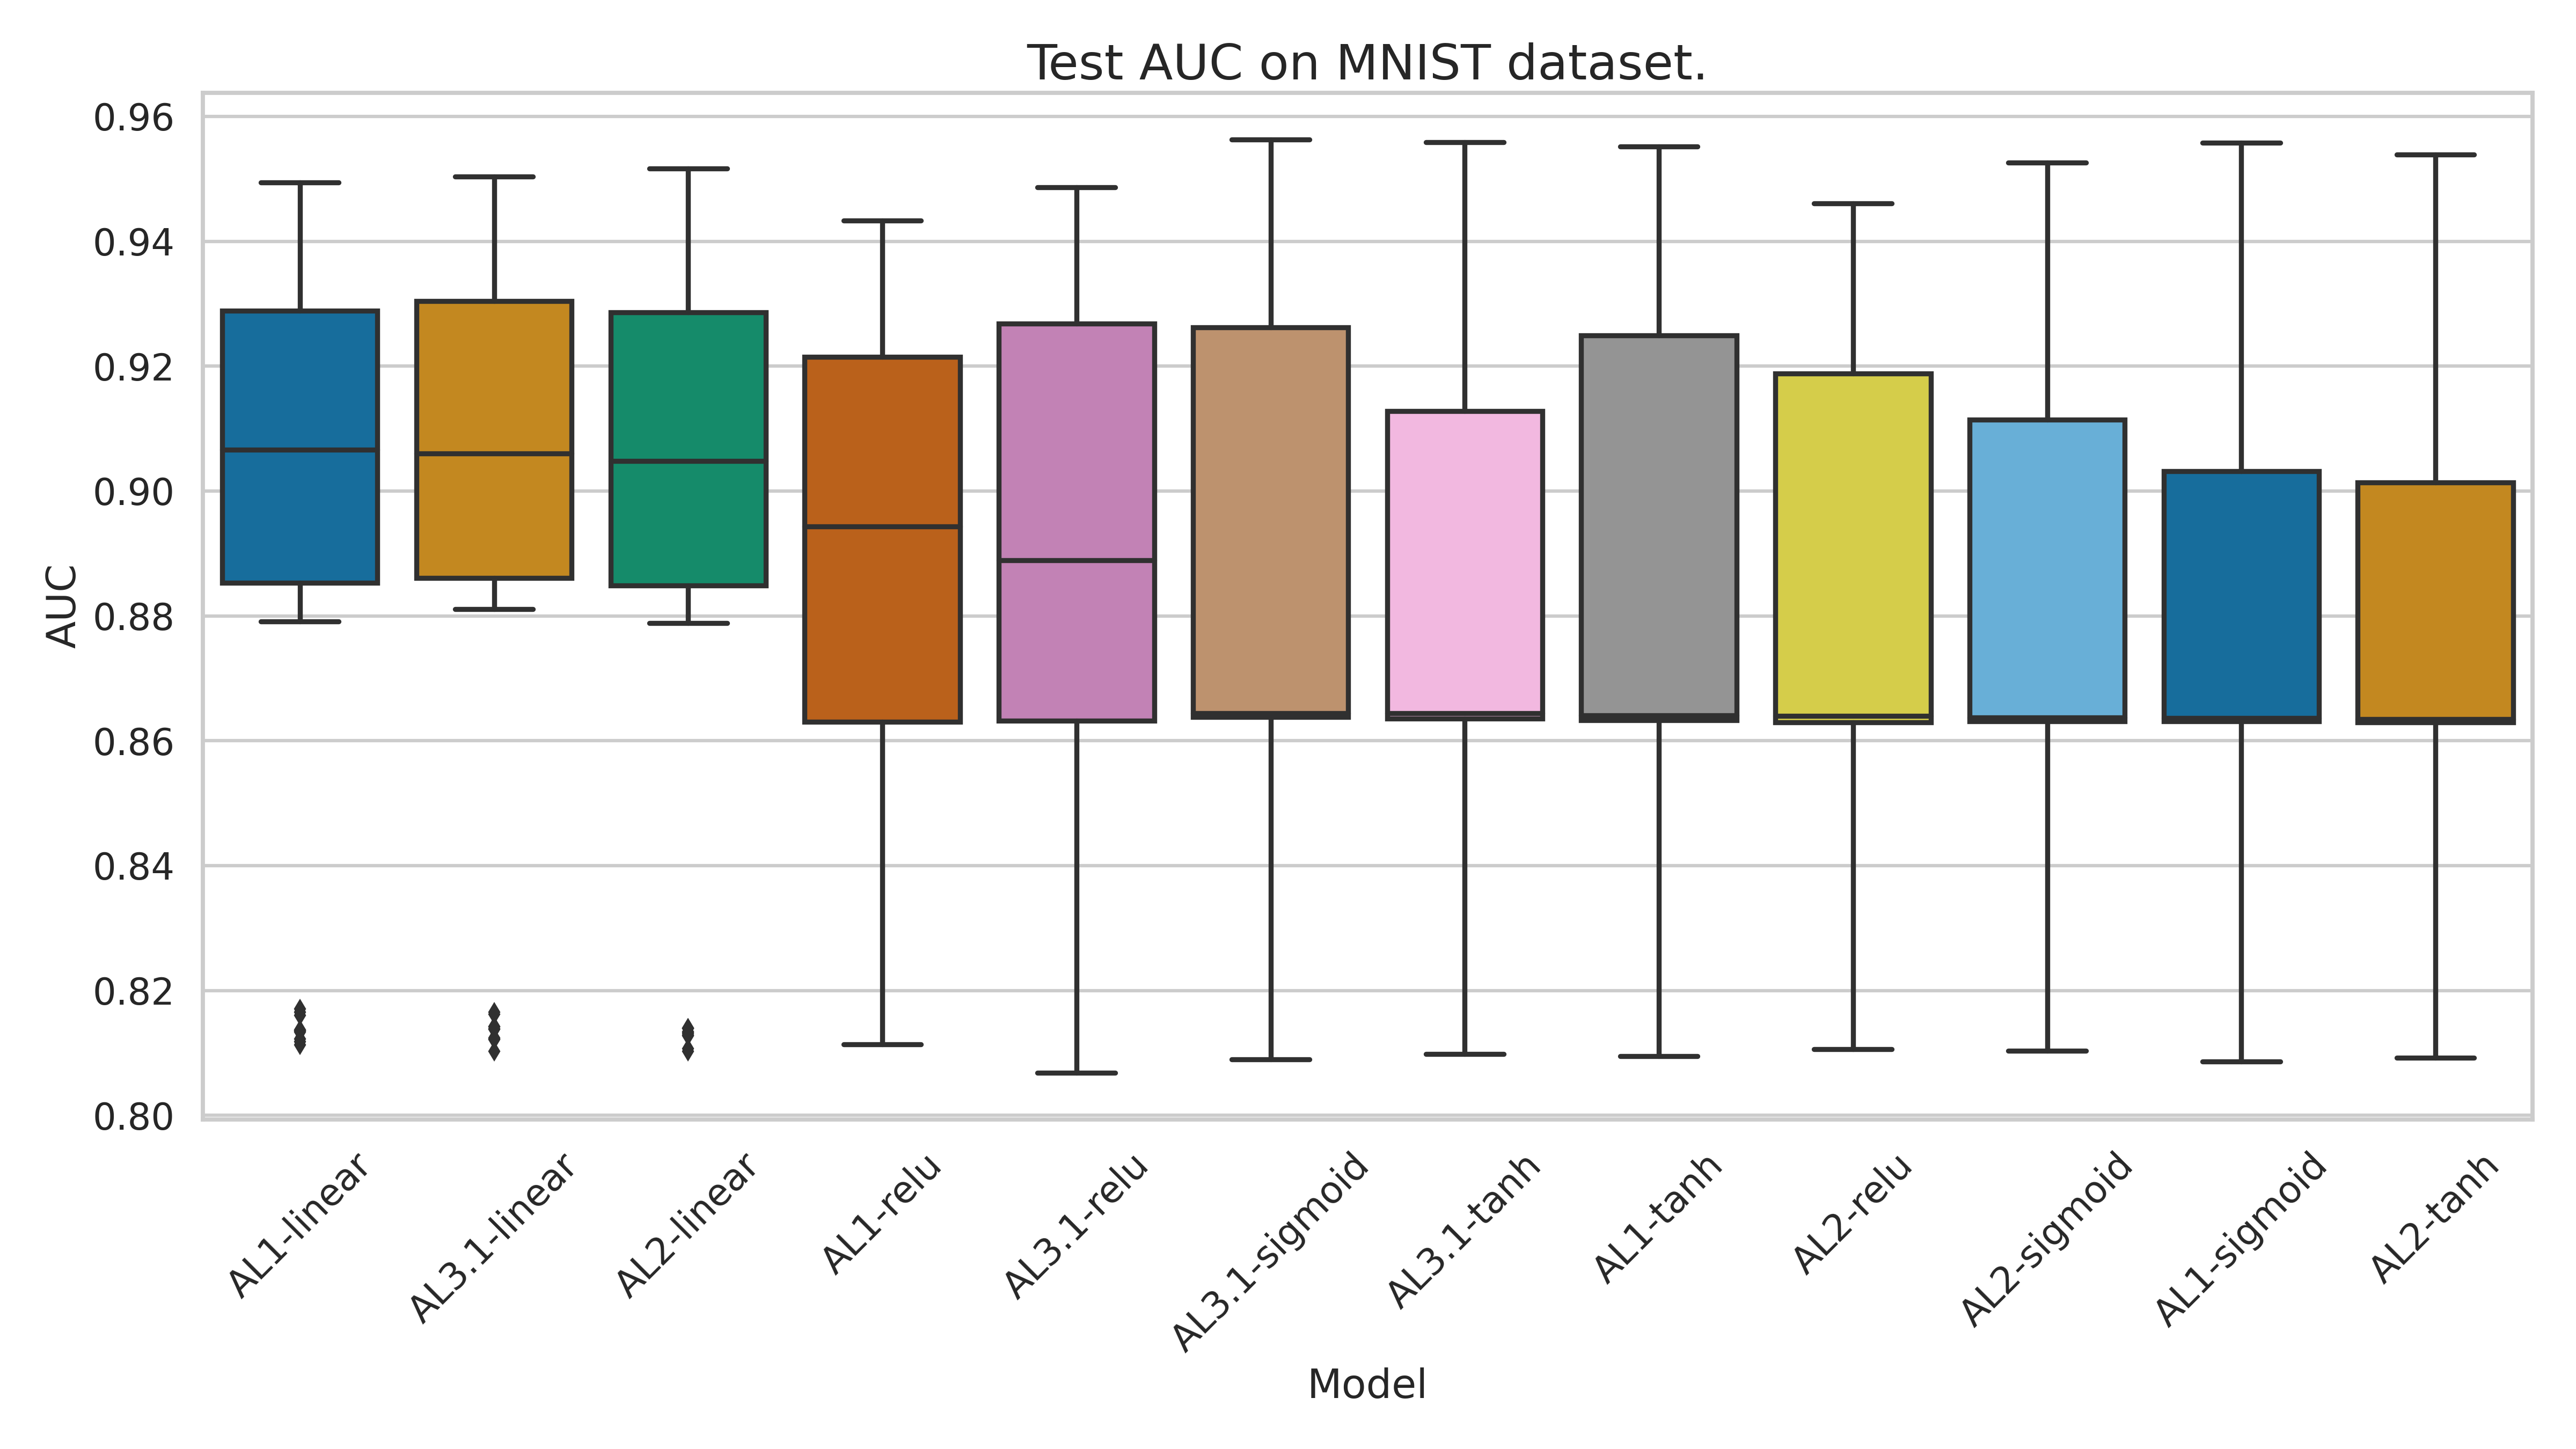
\includegraphics[width=\textwidth]{img/results/test_act.png}}
                \caption{Test AUC for the bottleneck activation function experiment on the MNIST dataset.}
                \label{fig:activation_test}
            \end{figure}
            
        \subsection{Data split}
            Once the bottleneck size and the bottleneck activation are found, the next step is finding the best partition sizes for the task.
            
            The experiment is conducted by performing 10 runs of models with different bottleneck data splits. For simplicity, we limited the experiment only to the approaches $AL1$, $AL2$, and $AL3$.
            
            We try the following splits:
            \begin{enumerate}
                \item 100 ($|A| = 50$, $ |B| = 50$, $|C| = 100$)
                \item 200 ($|A| = 100$, $ |B| = 100$, $|C| = 200$)
                \item 400 ($|A| = 200$, $ |B| = 200$, $|C| = 400$)
                \item 1000 ($|A| = 1000$, $ |B| = 1000$, $|C| = 2000$)
                \item 2000 ($|A| = 2000$, $ |B| = 2000$, $|C| = 4000$)
            \end{enumerate}
            
            The results of this experiment are shown in \autoref{fig:split_minst}. Based on the obtained results, we choose to use a data splitting of $1000$ images for the partitions $A$ and $B$ and $2000$ images for $C$.
            \begin{figure}[H]
                \centering
                \centerline{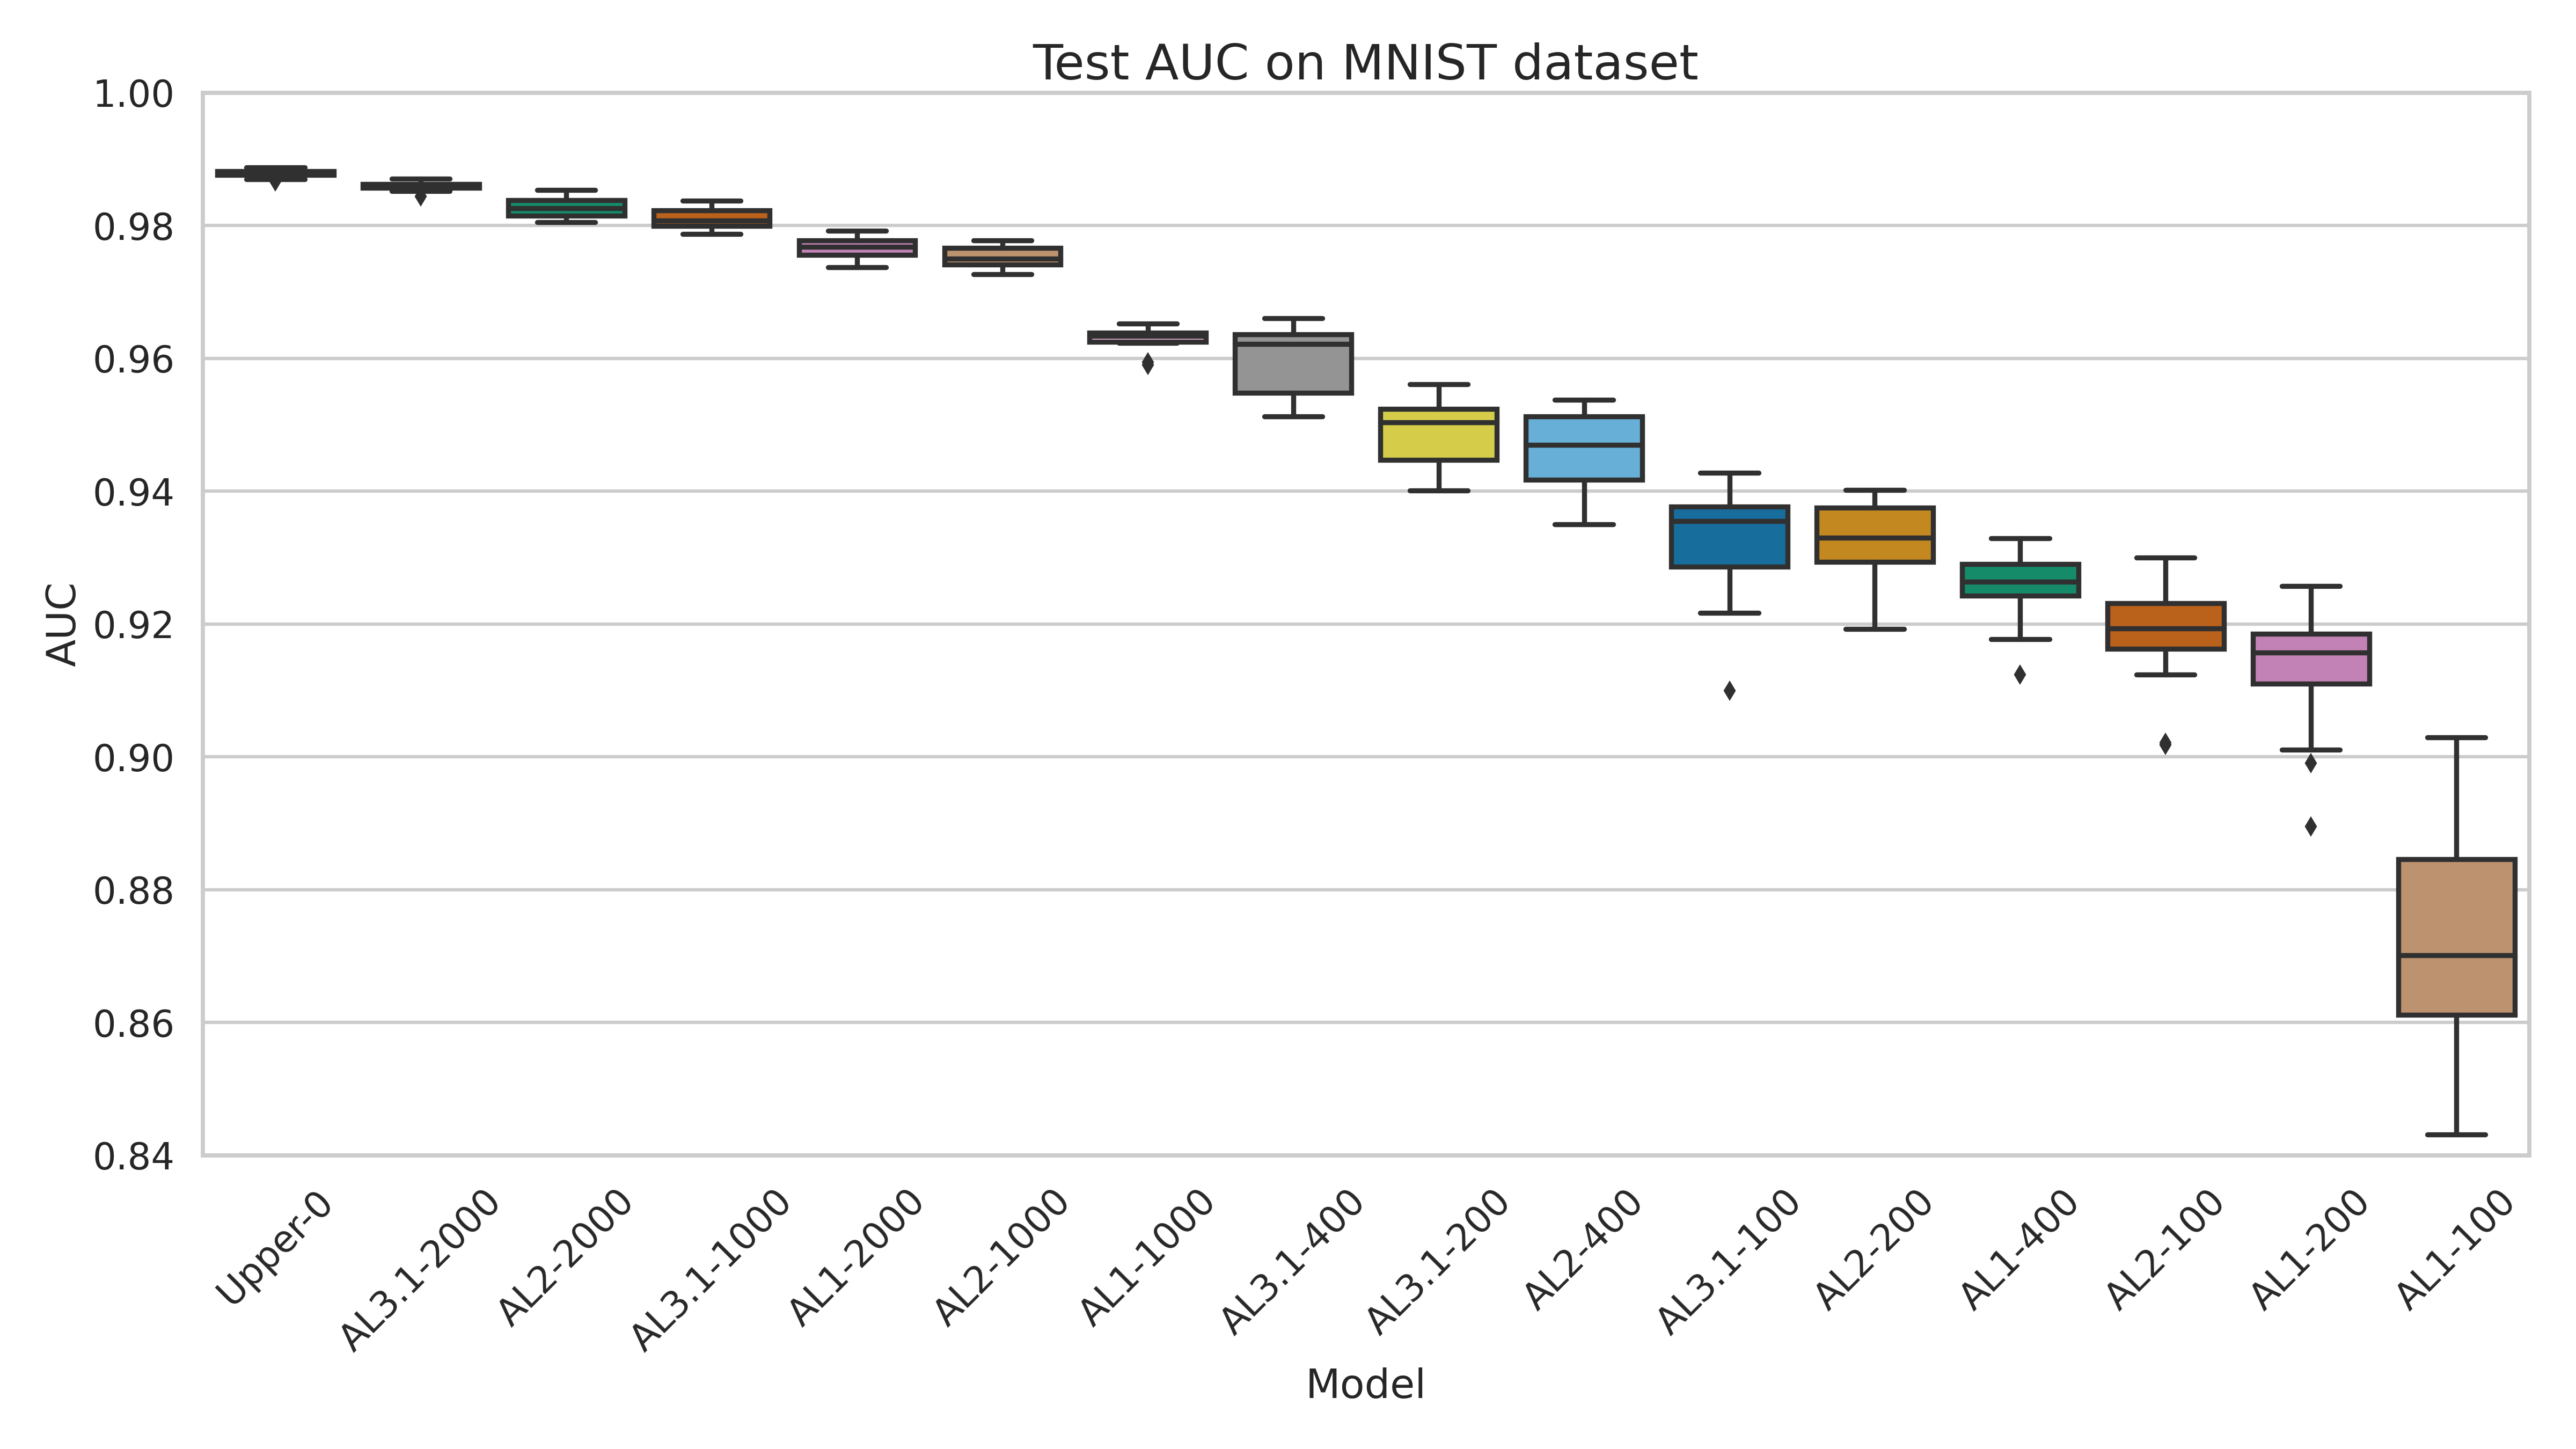
\includegraphics[width=\textwidth]{img/results/split_MN.png}}
                \caption{Test AUC for the partition size experiment on the MNIST dataset.}
                \label{fig:split_minst}
            \end{figure}

    \section{Experiments on the Hazards\&Robots dataset, Corridors scenario}
        Similar experiments are conducted on the real-life Hazards\&Robots dataset, Corridors scenario. This dataset is larger than MNIST, thus experiments require more time. Because of this, experiments in this section are not as broad as on the \emph{proxy} task.
        
        
        For the following experiments we perform \emph{data augmentation} along with resampling.
        
        We perform the following augmentation operations:
        \begin{itemize}
            \item Horizontal flip with a probability of 0.5;
            \item Random brightness contrast with a probability of 0.5, brightness and contrast limits of 0.1;
            \item Random crop with a probability of 0.5;
            \item Random rotation of maximum 10° with 0.5 probability.
        \end{itemize}
        \subsection{Early phase}
            In an early phase, we adapted the autoencoder to work with the images from the Hazards\&Robots, we then run some preliminary tests to check the correct function of the model (\autoref{fig:pred-rm}).
            
            \begin{figure}[H]
                \centering
                \centerline{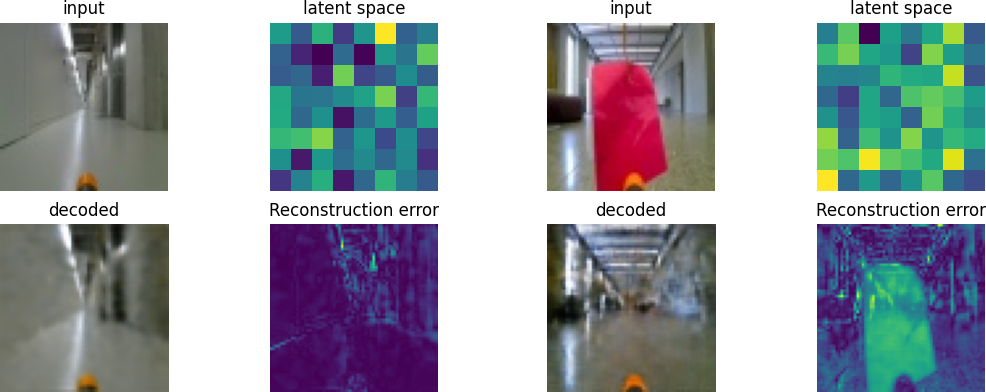
\includegraphics[width=\textwidth]{img/prediction_RM.png}}
                \caption{Example of predictions from a model trained on the Hazards\&Robots dataset. The input image on the left is from the normal class, while the other on the right is anomalous}
                \label{fig:pred-rm}
            \end{figure}
            
        \subsection{Bottleneck size}
            We choose to use a bottleneck size of 16 because Mantegazza et al~\cite{mantegazza2022sensing} in their experiments on this dataset show it performs better.
            
        \subsection{Data split}
            The next step is finding the best partition size for this task.
            
            Because of time constraints, since experiments on this dataset require more time than MNIST, we only try the following splits to $AL1$ only:
            
            \begin{itemize}
                \item 2 ($|A| = 1$, $ |B| = 1$, $|C| = 2$)
                \item 20 ($|A| = 10$, $ |B| = 10$, $|C| = 20$)
                \item 200 ($|A| = 100$, $ |B| = 100$, $|C| = 200$)
                \item 2000 ($|A| = 1000$, $ |B| = 1000$, $|C| = 2000$)
            \end{itemize}
            
            \noindent We choose to add to the comparison two more experiments: $AL1-2$, and $AL1-2000$ with no image augmentation.
            
            
            The results in \autoref{fig:split_rm} show how effective the data augmentation is when the training set is small, with $AL1-2$ outperforming its version with no augmentation. On the other hand, for the models with an initial training set of 2000 images, the augmentation led to a very small decrease in the model performance. We suppose this small decrease is due to noise introduced by the process of augmentation.
            
            
            We choose to use a data splitting of $1000$ images for the splits $A$ and $B$ partitions and $2000$ images for partition $C$.
            
            \begin{figure}[H]
                \centering
                \centerline{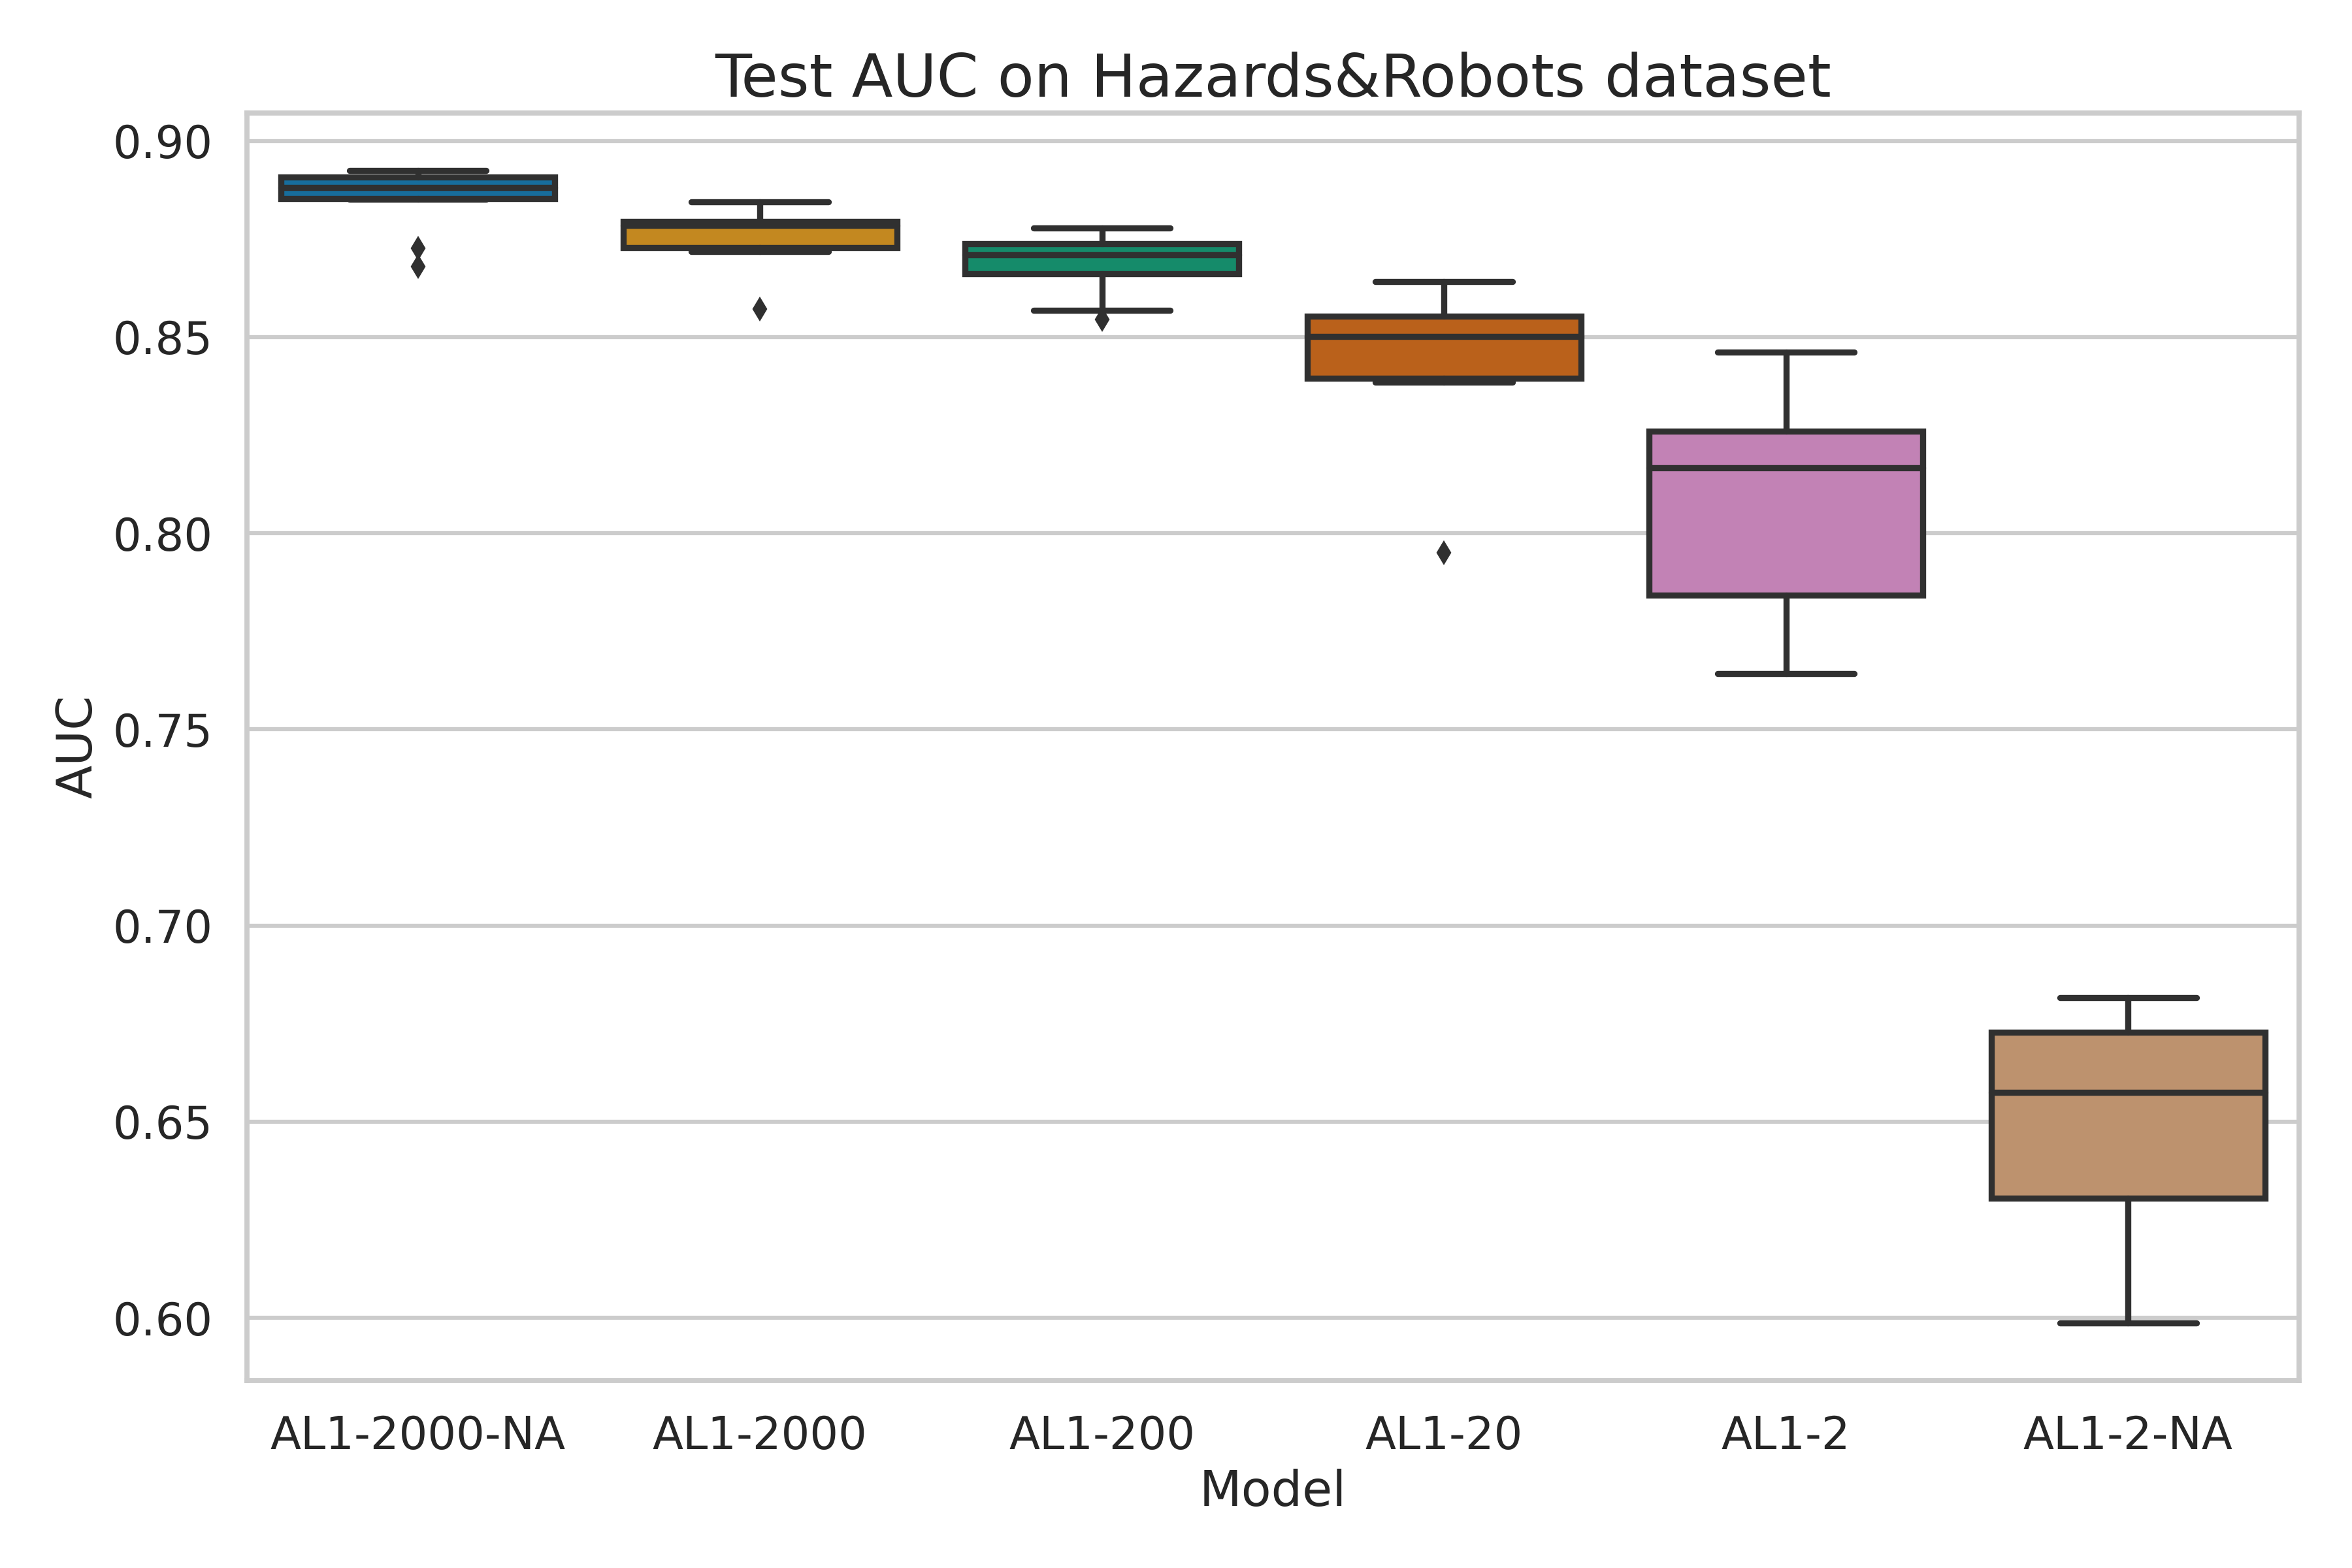
\includegraphics[width=\textwidth]{img/results/split_RM.png}}
                \caption{Test AUC on the Hazards\&Robots dataset for different data split.}
                \label{fig:split_rm}
            \end{figure}
        
    \section{AL metrics comparison}
        Now we have the best bottleneck and data partition hyperparameters for both our tasks.
        The final experiments are conducted to test and compare the different \acrshort{al} approaches proposed in \autoref{sub:al}.
    
        \subsection{MNIST}
            The results of the final experiments on the proxy task are shown in \autoref{fig:comparison-MN}.
            From the chart, we notice that no $AL$ approach has outperformed the others in a significant way. We notice that even with the random approach there is a significant improvement over the baseline model ($AL1$). However, for this task, the \acrshort{al} approaches proposed do not provide any significant improvement over the random query method ($AL2$).
            
            We suppose this is because the MNIST dataset is too simple for this task, the model quickly learns which features to extract to correctly reconstruct the input. Thus finding clever solutions to query useful data for the model shows little to no improvements in this setup.
            
            \begin{figure}[H]
                \centering
                \centerline{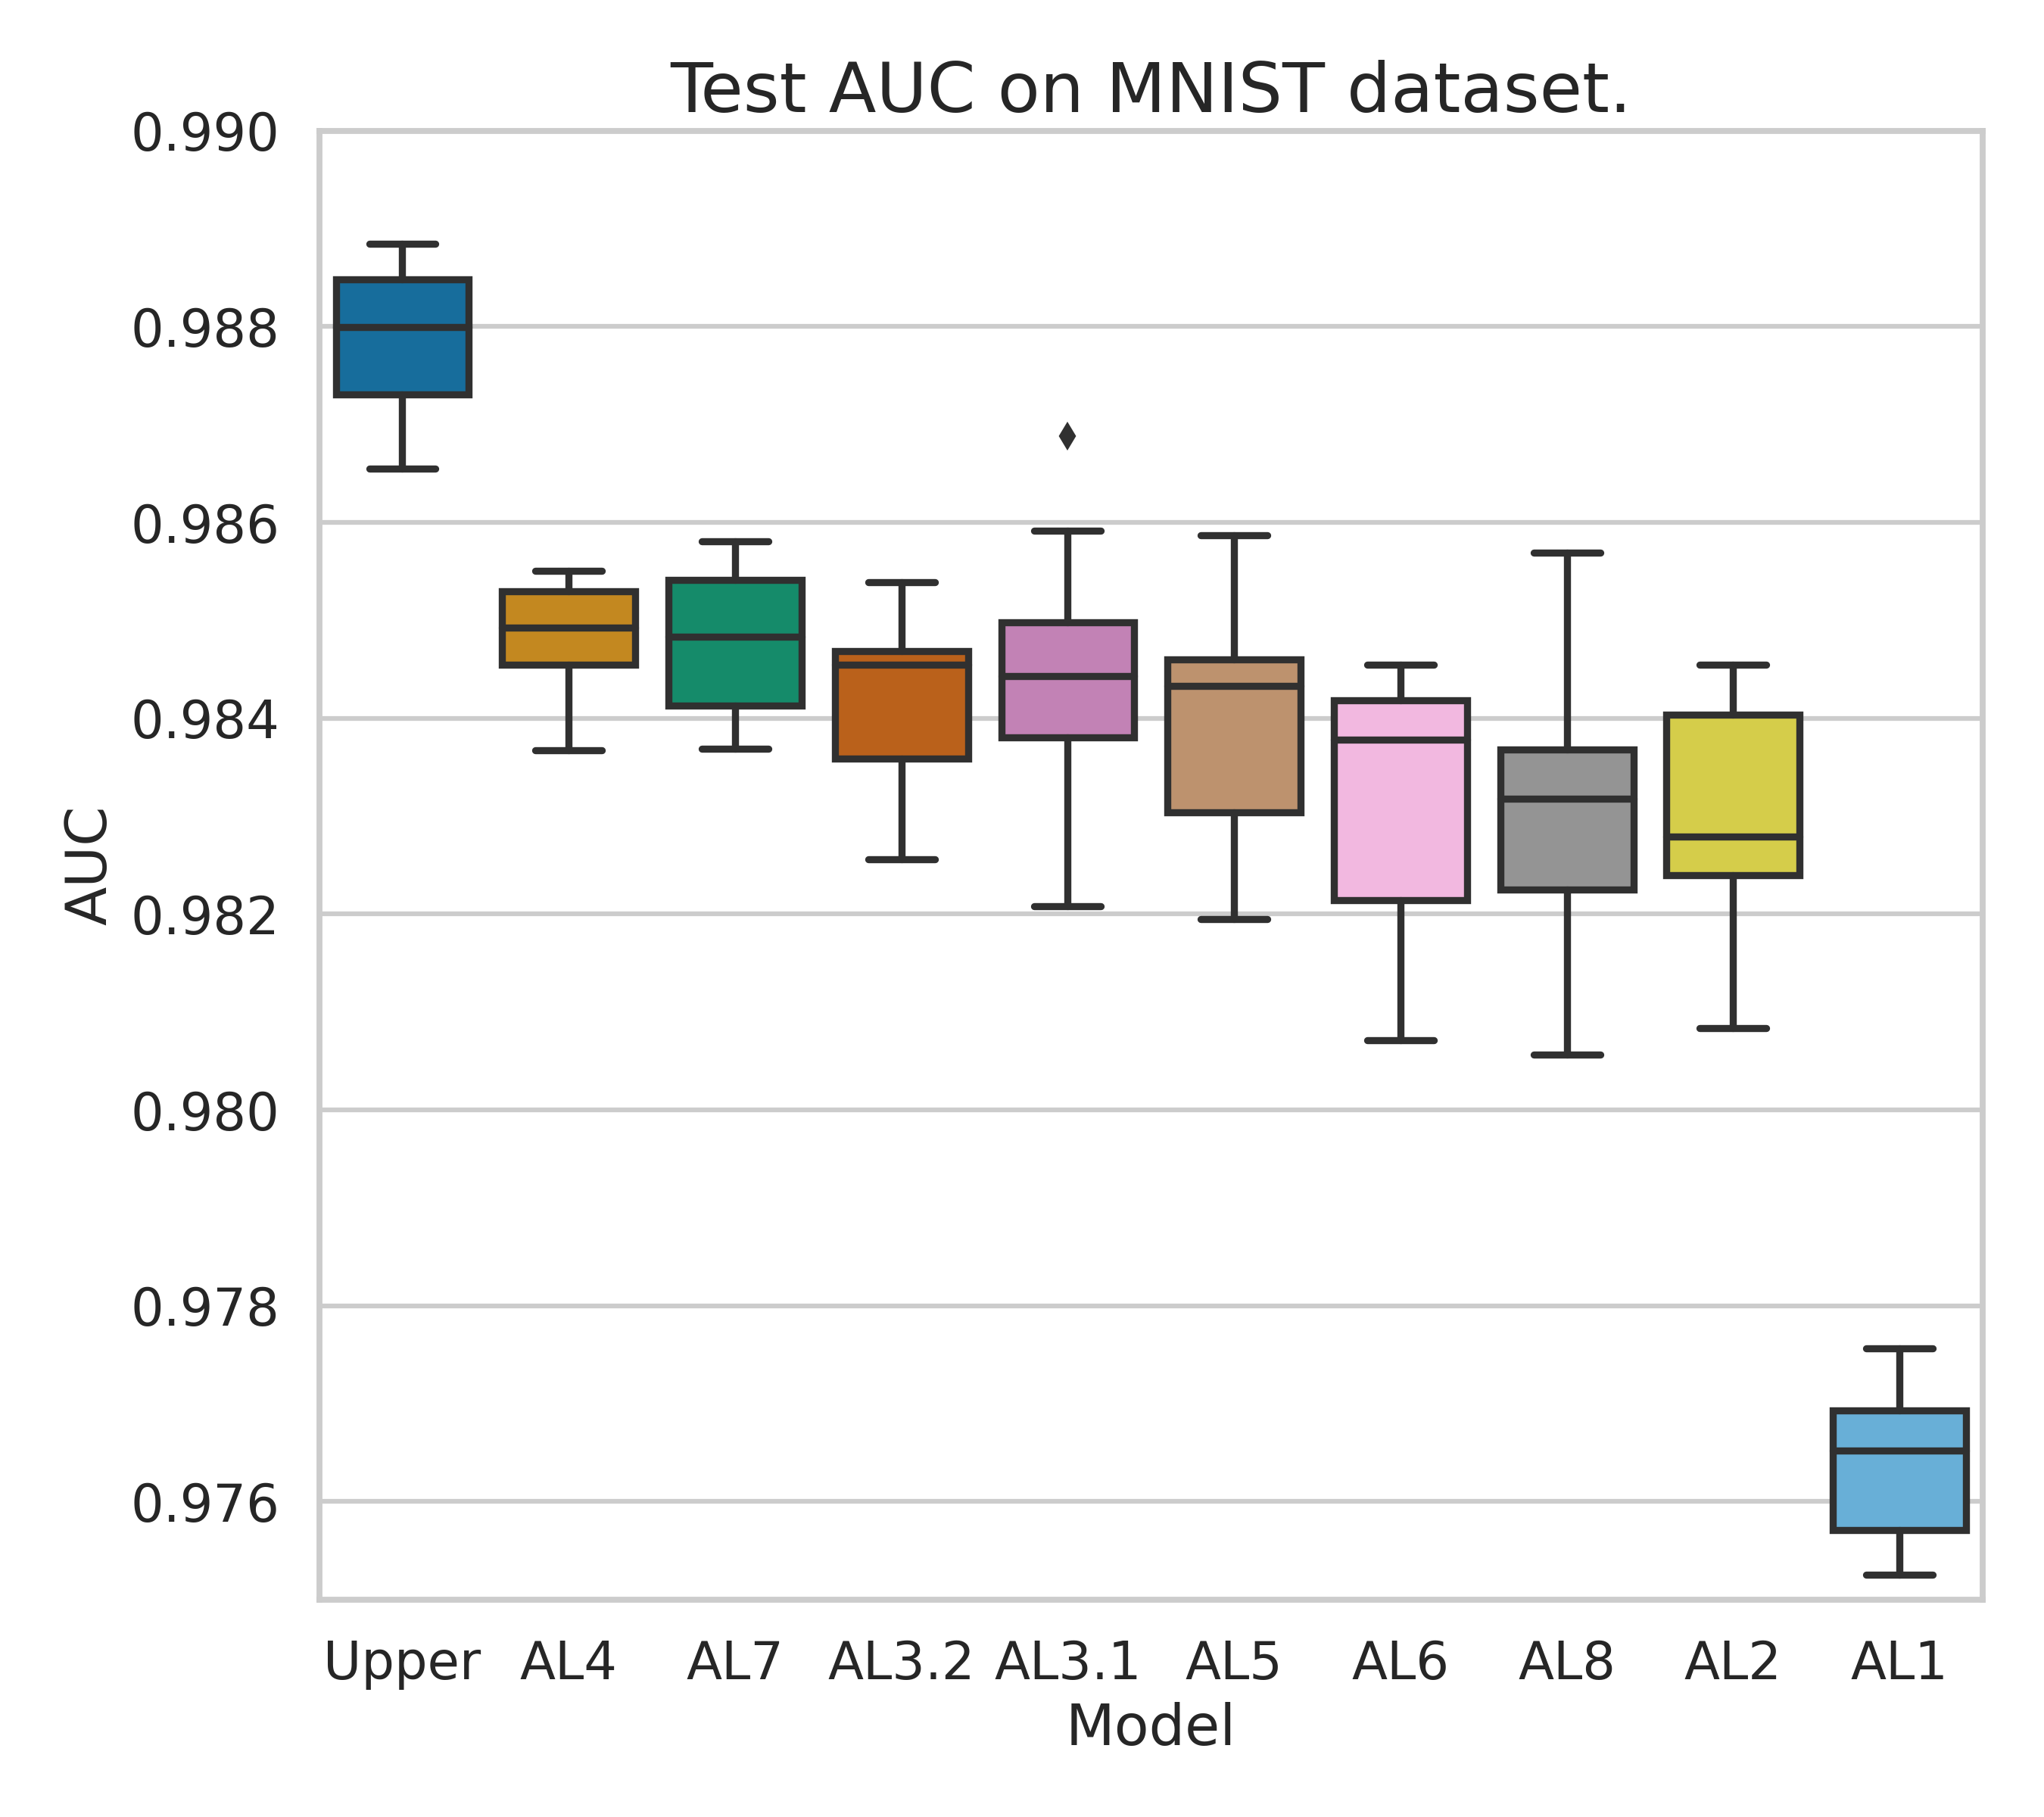
\includegraphics[width=\textwidth]{img/results/final_MNIST.png}}
                \caption{Test AUC on final experiments on the MNIST dataset}
                \label{fig:comparison-MN}
            \end{figure}
        
        \subsection{Hazards\&Robots dataset, Corridors scenario}
            The results of the final experiments on the Hazards\&Robots dataset, Corridors scenario are shown in \autoref{fig:comparison-MN}.
            
            
            From this real-life dataset, the results show a different pattern. We still have significant improvements with any model compared to the baseline. However, in this case, we have some models outperforming the random. More in detail, the approach $AL8$ outperformed both the baselines ($AL1$, $AL2$), scoring an \acrshort{auc} close to the upper bound of the dataset while using a training set of only 4,000 images.
            
            Another trend we notice is that methods that work on the \acrshort{ae}'s latent space show better performance than the ones which work in the image space.
            
            \begin{figure}[H]
                \centering
                \centerline{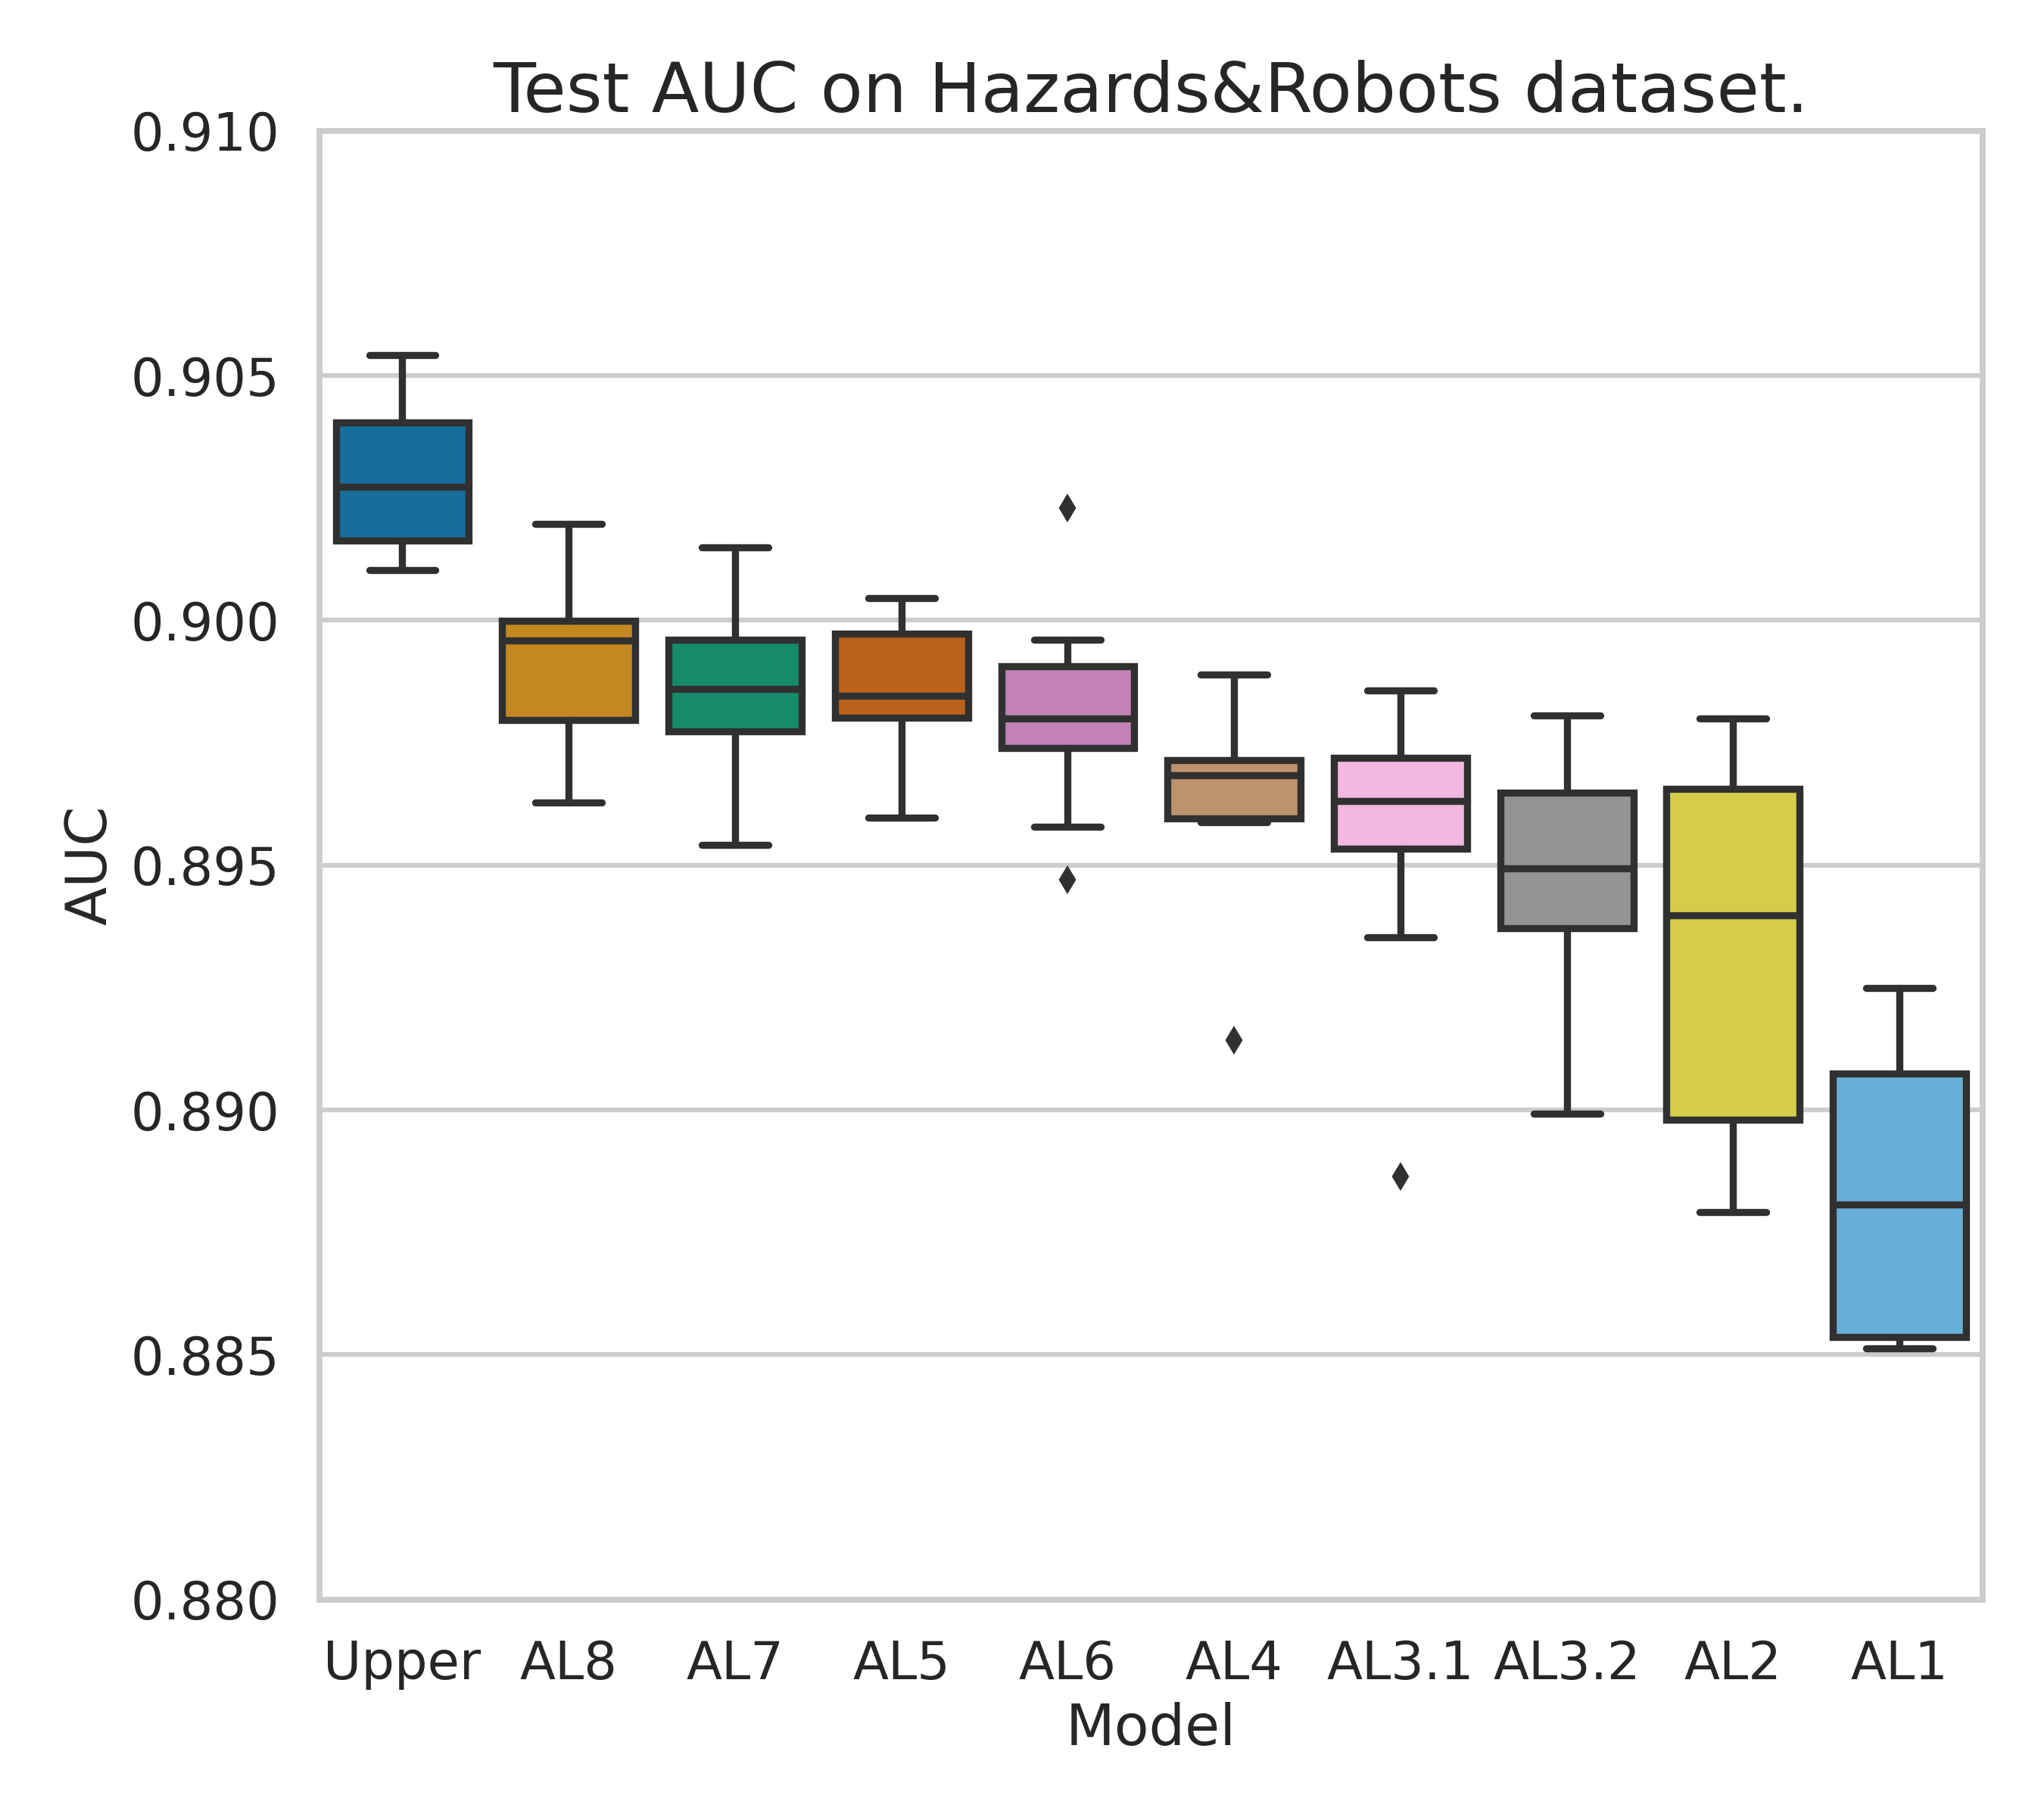
\includegraphics[width=\textwidth]{img/results/final_Hazards&Robots.png}}
                \caption{Test AUC on final experiments on the Hazards\&Robots dataset, Corridors scenario.}
                \label{fig:comparison-RM}
            \end{figure}
            
        \subsection{Comparison}
            We now directly compare the final results for both tasks. \autoref{fig:comparison} shows an overview of the \acrshort{auc} for both the MNIST dataset and the Hazards\&Robots dataset, Corridors scenario.
            
            We immediately notice that the results for MNIST are more "compact" when compared to our real-life dataset. This encourages our hypothesis that the MNIST dataset is way too simple for the task, nullifying the effort of performing \acrshort{al}.
            
            On the other hand, the chart of results on the Hazards\&Robots dataset, Corridors scenario shows how \acrshort{al} can be effective when applied to more complex tasks, leading to an \acrshort{auc} close to the upper bound using only a small fraction of the training data.
            \begin{figure}[H]
                \centering
                \centerline{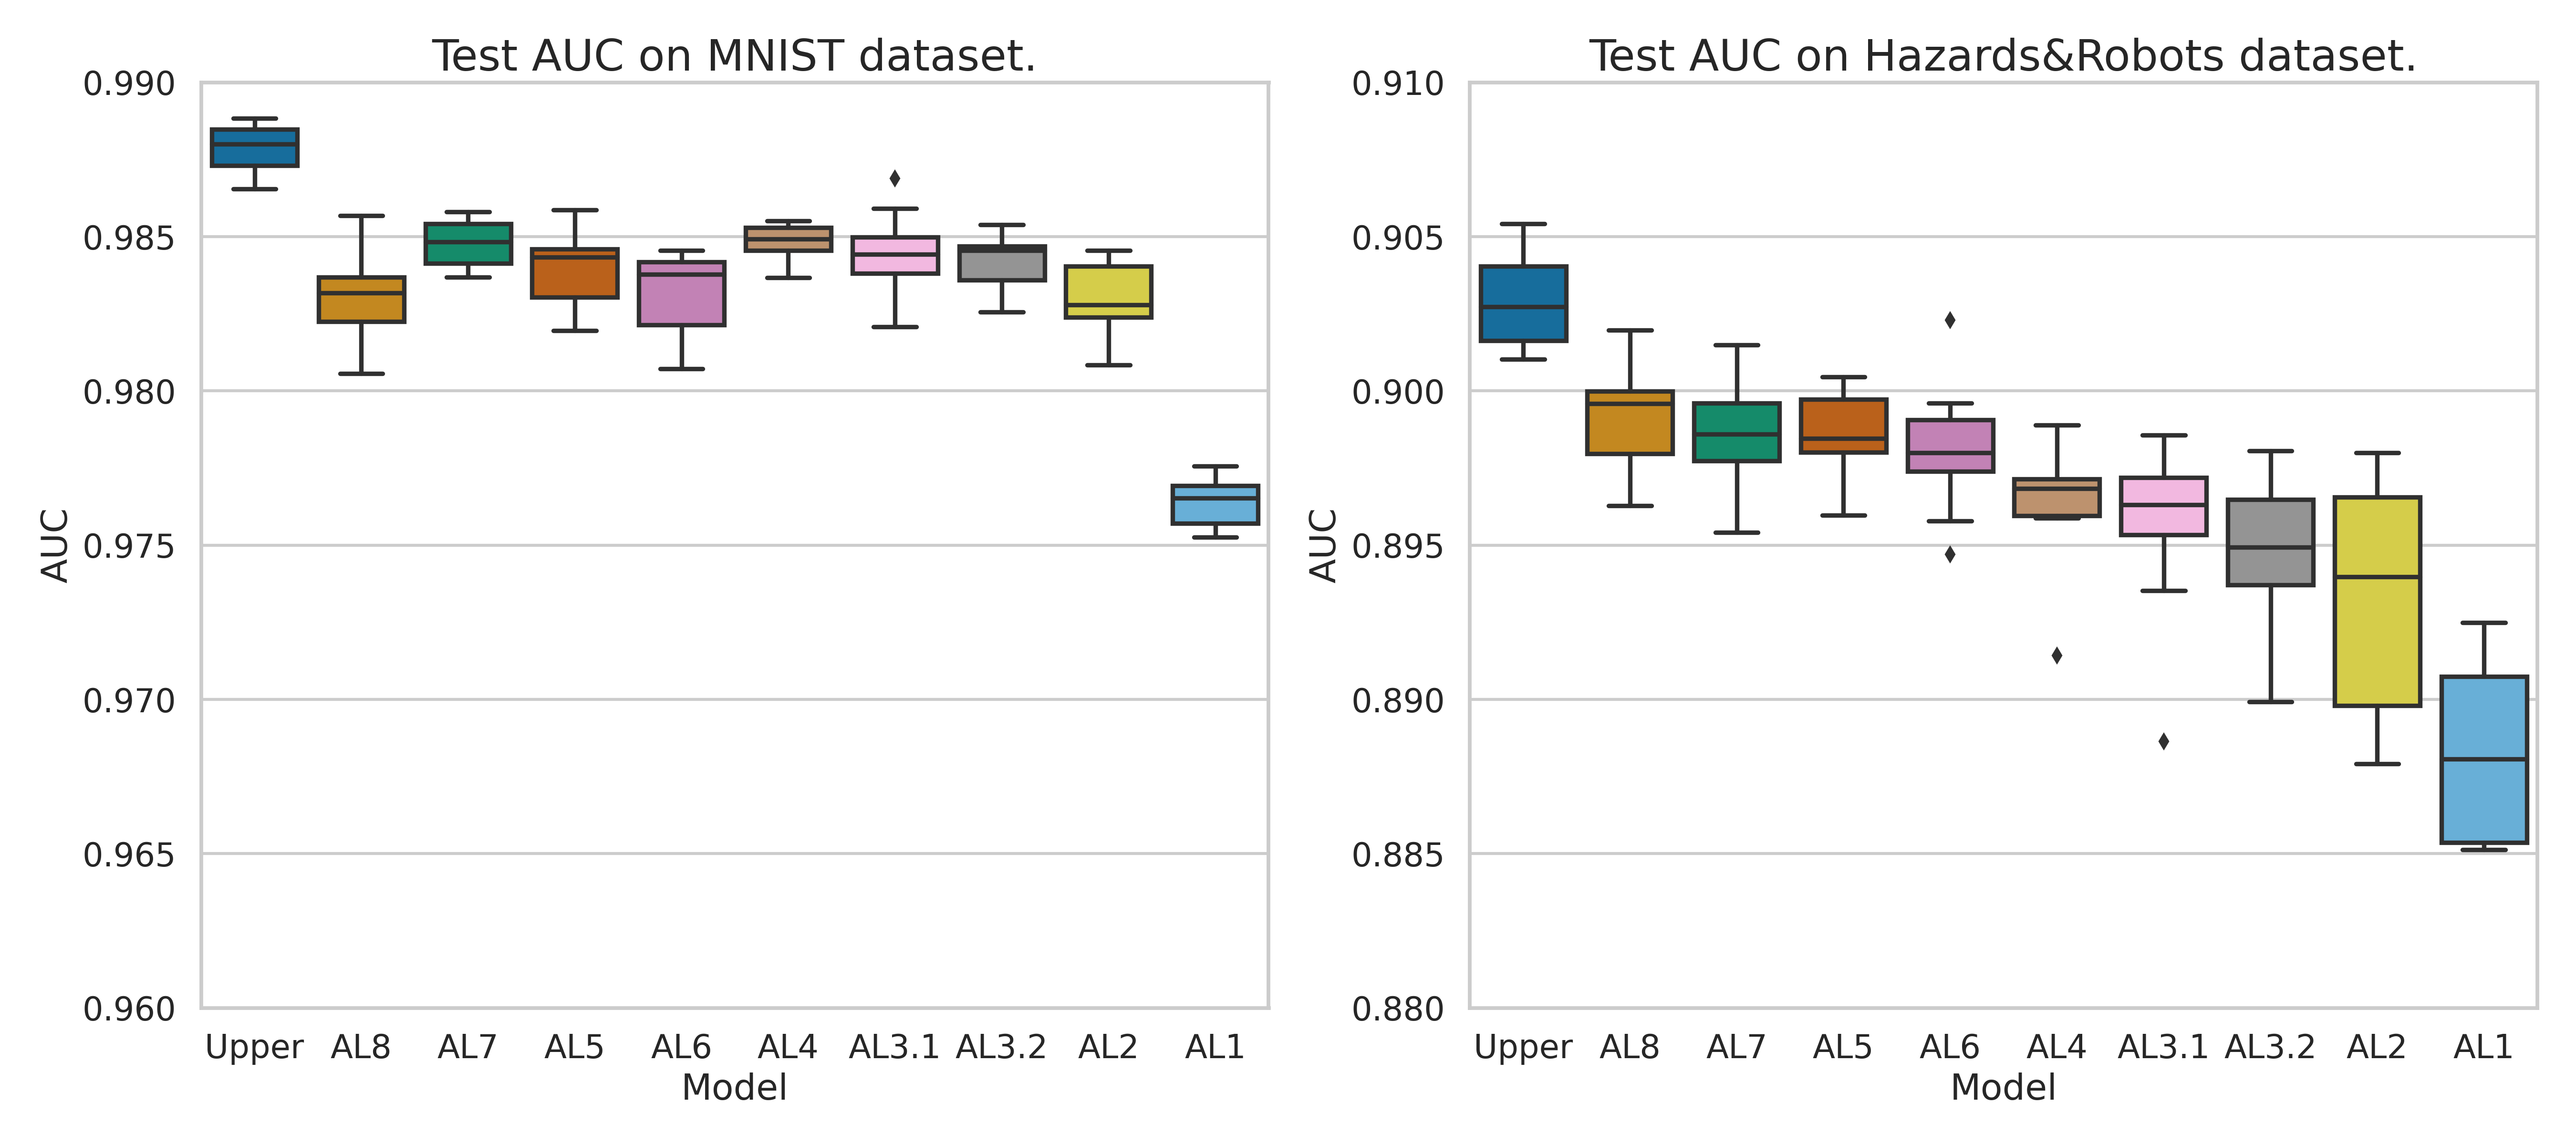
\includegraphics[width=\textwidth]{img/results/final_comparison.png}}
                \caption{Test AUC for final experiments. Comparison between MNIST and the Hazards\&Robots dataset, Corridors scenario}
                \label{fig:comparison}
            \end{figure}
            
        \subsection{Discussion}
        In this chapter we found the best bottleneck size, split size, and data split for both our tasks. We then tested the proposed \acrshort{al} approaches to both our datasets.
        
        
        \noindent We found out that for MNIST the best bottleneck size is 64, while 16 resulted the best for the Hazards\&Robots dataset.
        
        
        \noindent A linear bottleneck for the autoencoder leads to better performance then using an activation function.
        
        
        \noindent For both the datasets, the best split is 1000 images for partitions $A$ and $B$, 2000 for partition $C$.
        
        \noindent The approaches and the testing pipeline are validated using and testing some dummy models.
        
        \noindent As for the \acrshort{al} approaches, MNIST turned out to be way too simple for the task, with \acrshort{al} not providing any significant performance boost. On the other hand, on the Hazards\&Robots dataset the \acrshort{al} approaches which work in the latent space of the \acrshort{ae} outperformed the baselines and performed better than the \acrshort{al} methods which work in the image space.
        
        \noindent To summarize, \acrshort{al} applied the Hazards\&Robots dataset let us reach performance near to the upper bound by using only 4,000 samples.
        
        